%!TEX root = doe.tex

\section{Using the New Measure}
\label{sec:replications}

\note{Will need to rewrite this once the Reed stuff is in.}

We have shown that our measure, the DOE score, predicts international dispute outcomes better than the capability ratio.
But most recent studies of conflict do not aim to predict how disputes will end.
They focus on other dependent variables, and they usually only treat the capability ratio (or other functions of raw capabilities) as a control.
In this section, we investigate how well the DOE score performs as a replacement for the capability ratio in this more typical setting.
First, we replicate 18 recent empirical models of various international phenomena, finding that these models usually fit and predict better when we replace CINC-based measures with DOE scores.
After that, we provide some advice to practitioners on how to decide which measure---or measures---to include.

\subsection{What's New about Power?}

The DOE score's greatest potential lies in its ability to enhance tests of the role of power in international relations.
To that end, we begin our replication analysis by replicating a well-known test of the bargaining model.

\citet{reed2008war} provide an empirical examination of the bargaining model developed by \citet{powell1996stability,powell1999}.
The analysis focuses on two important parameters:  the probability that one state would prevail over the other in a conflict, $p$, and the distribution of benefits between the two states, $q$.
For example, $q$ may capture where a border is drawn between two neighboring states, though this animation is not necessary.
\citet[258]{powell1996stability} derives\footnote{%
  The probability here is equivalent to Powell's but uses the same expression as Reed et al. to simplify explication.
}
the equilibrium probability of conflict as
\begin{align*}
  \pi(p, q) &= \begin{cases}
  |q - p| - (q - p)^2, & |q - p| \leq \frac{1}{2} \\
  \frac{1}{4}, & |q - p| \geq \frac{1}{2}
  \end{cases},
\end{align*}
and Reed et al. provide a direct test of this expression by incorporating proxies of $|q - p|$ and $(q - p)^2$ (lagged one year) into a model of dispute onset.
They develop a new measure of $q$ based on United Nations roll call votes, and their measure of $p$ is a normalized cousin of the capability ratio based on the differences in CINC scores.\footnote{%
  For details on their measure of $p$, see footnote 11 of \citet[1211]{reed2008war}.
}
Our goal here is to replicate their results and then to estimate a faithful parallel model that uses DOE scores, rather than CINC scores, to proxy for $p$ while keeping all other covariates, including the Reed et al. measure of $q$, the same.

The first task is to assess the similarities of the two proxies of the two variables.
We plot the kernel densities of the measures in Figure \ref{fig:rcnw-measures}.
\begin{figure}[!ht]
  \centering
  \input{fig-rcnw-measures.tex}
  \caption{Comparison of Reed et al. (2008) and DOE proxies of $|q - p|$ and $(q - p)^2$.}
  \label{fig:rcnw-measures}
\end{figure}
Here the left column depicts $|q - p|$ and the right column depicts $(q - p)^2$.
The reader will note that the distributions are generally very similar, with nearly identical extrema, centralities, and dispersions.
The two absolute differences correlate at around~0.962, while the two squared differences correlate at around~0.957.
The average difference in the $|q - p|$ measures is~$-0.009$, and the average difference in the $(q-p)^2$ measures is~$-0.008$.
Suffice to say, the DOE versions of the two power variables are quite similar to those employed by Reed et al., which is not all that surprising given that we are using the same measure of $q$ for their construction.

Despite this strong similarity, Table~\ref{tab:rcnw}, which summarizes the results of our replication and DOE extension, reflects real differences.
\begin{table}[!ht]
\centering
\input{tab-rcnw.tex}
\caption{%
  Replication of Table 1, Model 2 of \citet[1213]{reed2008war}.
  The unit of analysis is the dyad-year, and the dependent variable is the onset of a militarized interstate dispute.
  The proportional reduction in loss over the constant-only model comes from 100 repetitions of 10-fold cross-validation.
}
\label{tab:rcnw}
\end{table}
We first turn our attention to the models' fit, captured by the \citet{Akaike:1974ih} Information Criterion (AIC),\footnote{%
  Using the \citet{Vuong:1989uf} test to assess in-sample fit of these non-nested models, we obtain a test statistic of~6.76, yielding a $p$-value under the null of identical fit of $7 \times 10^{-12}$.
} and predictive performance, captured by the proportional reduction in loss relative to a constant-only model (PRL).
The DOE replication outperforms the CINC-based model on both fronts, though the improvement in out-of-sample predictive performance is admittedly small.
Accordingly, we feel comfortable moving on to compare the substantive differences between the two models, should any exist.

And substantive differences indeed emerge.
The coefficient for the absolute difference of benefits and power remains positive, but it is more than halved in terms of its magnitude.
Meanwhile, the coefficient for the squared difference changes signs from negative to positive, increases in magnitude, and attains statistical significance at conventional levels.
(The same pattern holds in our replication of Reed et al.'s simpler Model 1, which we do not report here, but where the improvement in fit is even larger.)
Unsurprisingly, these changes transpire while the other coefficients remain nearly identical in their magnitudes and associated inferences.

These results refine, rather than refute, the extant arguments.
The point is best made visually; see Figure \ref{fig:rcnw}, which replicates Figure 2 (theoretical expectations) and Figure 4 (empirical results) from \citet[1207 and 1213, respectively]{reed2008war}.
\begin{figure}[!ht]
\centering
\input{fig-rcnw-gull.tex}
\caption{%
  Replication of Figure 4 of \citet[1213]{reed2008war}, which provides the predicted probability of MID onset as a function of the distribution of power (horizontal axis) and the distribution of benefits (vertical facets).
  Standard errors obtained via a parametric bootstrap.
}
\label{fig:rcnw}
\end{figure}
It remains that conflict becomes more likely as the distributions of benefits and power diverge, as we would expect given the positive coefficient for the $|q - p|$ term.
The difference here lies in the shape, and in particular in the persisence of the ``vee'' shape regardless of context.
What's more, the effect of the difference between benefits and power increases, rather than decreases, as the gap widens.
Whereas \citet[1206--1207]{reed2008war} suggest that context determines whether the probability of war follows a balance of power or preponderance of power pattern, our analysis suggests that the shape, though not the location, of the probability curve always supports the balance of power school.\footnote{%
  \citet[104--110]{powell1999} explicitly rejects both the Balance of Power and the Preponderance of Power schools because both schools minimize the probablity of conflict at a value---be it 0, $\frac{1}{2}$, or 1---that is independent of the distribution of benefits, $q$.  
}
It is interesting that when distribution of benefits is moderate (that is, in the $q = 0.5$ row), the predicted probabilities from the two models are virtually identical.
However, in each of the other two rows, which depict the situation when the benefits are not distributed so equitably, we notice a difference in the shape of the predicted probability plots.
Consider the top row, where $q = 0.1$. 
Toward the right edge of both panels, the balance of power is severely shifted in State $A$'s favor, which induces a dissonance with the distribution of benefits, which favors State $B$.  
Using the CINC-based proxy for $p$, the effect of that dissonance is decreasing; indeed, at the very right edge of the plot, the predicted probabilities again turn \emph{downward}, albeit only slightly so.
We think it makes intuitive sense that we should expect largerrisk of conflict as the distributions of power and benefits become more dissonant, as the DOE analysis suggests, rather than that the probabilities flatten out (as Powell's theoretical model suggests) or even that they turn downard (as Reed et al.'s empirical model suggests).



\subsection{Capabilities as Control}

In dyadic analyses of conflict, the capability ratio is usually included as a control variable, not one of the independent variables of interest.
Even when power is not a study's main focus, it is important to use the best available proxy for power.
Unless dyadic power relations have no effect on the outcome of interest (in which case proxies for power do not belong in the model), better proxies will capture more residual variation, resulting in greater model fit and more precise inferences.
And if power is a confounding variable---i.e., power relations are correlated with both the key independent variable and the outcome---then the bias of the estimated relationship will be inversely related to the quality of the proxy.
Reducing variance and bias are key concerns for any empirical analyst, so proxy quality matters.

To compare the performance of the DOE score as a control variable to that of the capability ratio, we replicate 18 recent analyses of conflict.
In each replication, we rerun the main model with DOE scores in place of the capability ratio (or other CINC-derived proxy for relative power).
Our main concern is fit: do the models with the DOE score capture more of the variation in the outcome of interest than those with the capability ratio?
In 14 out of 18 cases, the answer is yes, indicating that DOE scores make for a better control variable in typical statistical analyses of conflict.

We constructed the set of replications by looking for empirical analyses of dyad-years (directed or undirected) that included the capability ratio or another function of CINC scores as a covariate.
Each study was published recently in a prominent political science or international relations journal.\footnote{%
  For details, see footnote~\ref{fn:journals}.
}
We examined only studies with publicly available replication data.
If we could not reproduce a study's main result or were unable to merge the DOE scores into the replication data (e.g., because of missing dyad-year identifiers), we excluded it from the analysis.
We also excluded studies that employed duration models or selection models, due to conceptual and technical problems with assessing their out-of-sample performance.
Lastly, we excluded studies in which our measure of expected dispute outcomes would be endogenous, namely those whose dependent variable was MID outcomes---the same data we used to construct the DOE scores---or a closely related quantity.\footnote{%
  The dependent variable of each study is listed in the Appendix.
  In most cases it is the initiation or onset of a dispute.
}
In the end, we were left with the 18 studies listed in Table~\ref{tab:replications}.

For each analysis in our sample, we begin by identifying the main statistical model reported in the paper, or at least a representative one.\footnote{%
  When no main model is apparent, our heuristic is to pick one on the log-likelihood--sample size frontier.
  Details of the model chosen from each paper and the functions of CINC and DOE scores used are in the Appendix.
}
We then estimate two models: the original model, and a replicated model where we replace any functions of CINC scores with their natural equivalents in DOE scores.
For example, if the capability ratio is logged in the original model, we log the DOE scores in the replicated model.
Our main measure of comparative model fit is the \citet{Vuong:1989uf} statistic for the test of the null hypothesis that the original and replicated models fit equally well.\footnote{%
  We employ the standard Bayesian Information Criterion \citep{Schwarz:1978kh} correction to the Vuong test statistic.
  We also measured model fit by the \citet{Akaike:1974ih} Information Criterion and repeated cross-validation; the results, which are reported in the Appendix, are essentially the same.
}

\afterpage{
  \clearpage
  \begin{landscape}
    \begin{table}[h]
      \centering
      \input{tab-replications}
      \caption{
        Summary of results from the replication analysis.
        Positive values of the Vuong test statistic indicate that the model with DOE terms fits better than the model with CINC terms, and vice versa for negative values.
        The next two columns report whether $p < 0.05$ for the main substantive hypothesis test under each model; the final two report whether $p < 0.05$ for a test of the null hypothesis that all power variables have a coefficient of zero.
      }
      \label{tab:replications}
    \end{table}
  \end{landscape}
}

We are also interested in how DOE scores change our inferences about the main substantive variables or about the effect of power itself.
We identify the main substantive hypothesis of each study and perform the corresponding null hypothesis test on both the original model and the DOE score replication.
The hypotheses tested are listed in the Appendix.
To test for an effect of relative power, in the original models we test the null hypothesis that all CINC-derived terms have a coefficient of zero, and in the replication models we do the same with the DOE terms.

Table~\ref{tab:replications} summarizes the results of the replication analysis.
The results further support our contention that DOE scores are superior to the capability ratio as a proxy for relative power.
In a majority of the conflict studies we replicate, we explain more of the variation in the dependent variable when we replace the capability ratio with DOE scores as a control for power.
According to the Vuong statistic, the DOE model fits better in 14 out of 18 cases; in six of these, the difference is statistically significant (the Vuong statistic exceeds 1.96).
These results reinforce our confidence in the DOE score's quality as a proxy for relative power.
They also affirm our conceptualization of relative power as the expected outcome of a dispute: by optimizing for dispute outcome prediction, we end up with a measure that is better for modeling a variety of other outcomes as well.

In most of the replications, the main substantive inference does not depend on the measure of relative power.
That is not surprising, given that power is only a control variable in these studies.
There are, however, two exceptions---studies for which the DOE model fits better and nullifies the statistical significance of the main substantive hypothesis.
Both are analyses of the international ramifications of domestic politics.
The first is the study by \citet{Arena:2009gk} examining the effects of major powers' government partisanship and economic conditions on their propensity to initiate disputes.
The original study measures capabilities by the initiating state's CINC score.
When we substitute in DOE scores, we find that the model fits significantly better, yet we can no longer reject the null hypothesis that government partisanship has zero effect (Wald $\chi^2 = 6.62$, $\text{df} = 8$, $p = 0.58$).\footnote{%
  The null hypothesis is that government partisanship and its three interactions with economic variables has zero coefficient in both the mean and dispersion equations.
  See the Appendix for details.
}
The second is \citeapos{Jung:2014jq} analysis of diversionary conflict.
The original study includes both the capability ratio and a CINC-based measure of rising powers; it interacts the latter with domestic unrest, a key independent variables of interest.
When we replace the capability ratio and the rising power measure with their DOE score equivalents, the resulting model fits better (though not statistically significantly per the Vuong test), and domestic unrest and its interaction with rising power are jointly insignificant (Wald $\chi^2 = 3.46$, $\text{df} = 2$, $p = 0.18$).
By using a weak proxy for relative power, both of these analyses fail to pick up its confounding effects on the relationship of interest, leading them to overstate the effects of domestic pressures on international conflict.

The most striking results of the replication analysis come from the tests of the effects of power.
In a third of the original studies, the relative power variables are statistically insignificant.
One might conclude from these results that the importance of material power to international conflict is not robust.
However, the DOE variables are jointly significant in every one of the replicated models.
The insignificance of the capability ratio in many studies is not because power is unimportant, but because the capability ratio is such a poor proxy for power.


\subsection{Advice to Practitioners}

Seeing as neither the capability ratio nor DOE scores are uniformly better in typical applications, how should empirical scholars choose which one to include in their analysis?
Our main recommendation is a theory-driven approach.
When theory provides no guidance, we recommend either a data-driven approach or dropping capability measures altogether.

\begin{figure}[htp]
  \centering
  \input{dag-cap0-doe1}
  \caption{
    Raw capabilities only affect the outcome of interest through expectations.
  }
  \label{fig:dag-cap0-doe1}
\end{figure}

If theory suggests that material capabilities only affect the outcome of interest insofar as they shape expectations about how a dispute would end, then DOE scores are the best measure to control for.
Figure~\ref{fig:dag-cap0-doe1} contains a causal graph of this situation.
The clearest examples of theories where only expectations matter come from the formal literature on crisis bargaining.
Take \citeauthor{powell1999}'s~\citeyearpar{powell1999} theory of bargaining in the shadow of power.
War is possible only if the status quo distribution of benefits is far enough from the expected outcome of conflict that at least one state is dissatisfied.
An empirical model derived from this theory should control for DOE scores rather than the capability ratio or other poor proxies for expectations.

\begin{figure}[htp]
  \centering
  % Main document must include
% \usepackage{tikz}  % for the graphics
% \usepackage{etoolbox}  % for the if-then toggles

\providetoggle{cap-to-dv}
\providetoggle{doe-to-dv}

\toggletrue{cap-to-dv}
\toggletrue{doe-to-dv}

% Main document must include
% \usepackage{tikz}  % for the graphics
% \usepackage{etoolbox}  % for the if-then toggles

\providetoggle{cap-to-dv}
\providetoggle{doe-to-dv}

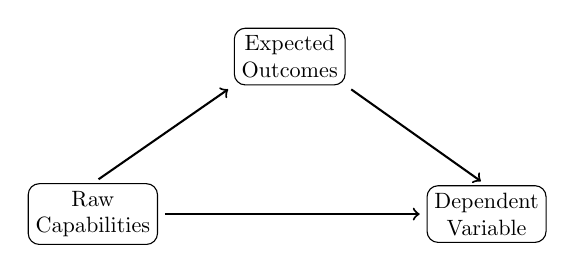
\begin{tikzpicture}[
  var/.style={
    rectangle,
    rounded corners,
    draw=black,
    align=center,
    scale=0.8
    }
  ]
  
  \node[var] (cap) at (0, 0) {Raw\\Capabilities};
  \node[var] (doe) at (2.5, 2) {Expected\\Outcomes};
  \node[var] (dv) at (5, 0) {Dependent\\Variable};

  \path[->, line width=0.75pt] (cap.north) edge[shorten <=0.25em, shorten >=0.25em] (doe.south west);
  \iftoggle{doe-to-dv}{\path[->, line width=0.75pt] (doe.south east) edge[shorten <=0.25em, shorten >=0.25em] (dv.north);}{}
  \iftoggle{cap-to-dv}{\path[->, line width=0.75pt] (cap.east) edge[shorten <=0.25em, shorten >=0.25em] (dv.west);}{}
\end{tikzpicture}

%%% Local Variables:
%%% mode: latex
%%% TeX-master: "doe"
%%% End:


  \caption{
    Raw capabilities affect the outcome of interest both directly and through expectations.
  }
  \label{fig:dag-cap1-doe1}
\end{figure}

If material capabilities affect the outcome both directly and indirectly via expectations, then it would be appropriate to control for both raw capabilities and expected dispute outcomes.
Figure~\ref{fig:dag-cap1-doe1} illustrates this scenario.
For example, imagine an empirical study of ``sinking costs'' via military mobilization in international crises \citep{fearon_signaling_1997}.
The initial movement of peaceful relations into a crisis, as well as early behavior at the bargaining table, might be shaped solely by states' expectations about dispute outcomes.
But if states build up their military as a way to signal resolve, independently of the effect on likely outcomes, then raw capabilities matter too.
When empirically modeling a theory like this, scholars should include both DOE scores and raw capability measures.
The ratio of CINC scores may or may not be the most appropriate way to capture raw capabilities---that, too, depends on the specifics of the theory.

\begin{figure}[htp]
  \centering
  % Main document must include
% \usepackage{tikz}  % for the graphics
% \usepackage{etoolbox}  % for the if-then toggles

\providetoggle{cap-to-dv}
\providetoggle{doe-to-dv}

\toggletrue{cap-to-dv}
\togglefalse{doe-to-dv}

% Main document must include
% \usepackage{tikz}  % for the graphics
% \usepackage{etoolbox}  % for the if-then toggles

\providetoggle{cap-to-dv}
\providetoggle{doe-to-dv}

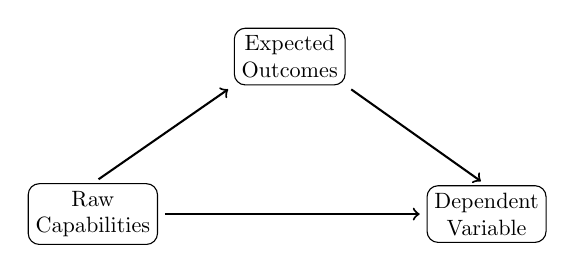
\begin{tikzpicture}[
  var/.style={
    rectangle,
    rounded corners,
    draw=black,
    align=center,
    scale=0.8
    }
  ]
  
  \node[var] (cap) at (0, 0) {Raw\\Capabilities};
  \node[var] (doe) at (2.5, 2) {Expected\\Outcomes};
  \node[var] (dv) at (5, 0) {Dependent\\Variable};

  \path[->, line width=0.75pt] (cap.north) edge[shorten <=0.25em, shorten >=0.25em] (doe.south west);
  \iftoggle{doe-to-dv}{\path[->, line width=0.75pt] (doe.south east) edge[shorten <=0.25em, shorten >=0.25em] (dv.north);}{}
  \iftoggle{cap-to-dv}{\path[->, line width=0.75pt] (cap.east) edge[shorten <=0.25em, shorten >=0.25em] (dv.west);}{}
\end{tikzpicture}

%%% Local Variables:
%%% mode: latex
%%% TeX-master: "doe"
%%% End:


  \caption{
    Raw capabilities directly affect the outcome of interest, but expectations do not.
  }
  \label{fig:dag-cap1-doe0}
\end{figure}

The last possibility to consider is that expectations do not affect the outcome of interest.
In this case, empirical models should only include raw capability measures, not DOE scores.
The clearest example is when the dispute outcome itself is the dependent variable.
First, absent some kind of self-fulfilling prophecy effect, we would expect actual capability holdings to drive outcomes more so than expectations.
Second, because DOE scores are calculated using the dispute outcome data, the DOE scores themselves are endogenous to observed outcomes, and thus should not be included as an independent variable when outcome is the dependent variable.\footnote{%
  In principle, this latter problem could be solved, albeit at great computational expense, by only using data for years up to $t-1$ to calculate the DOE score for year~$t$.
}

When there is no theory or the theory does not specify how material capabilities affect the outcome of interest, we recommend a data-driven approach.
The steps are the same ones we took in the replication analysis: determine a metric for model fit (whether in- or out-of-sample), run the model separately for each potential measure, and choose the best-fitting model.
Alternatively, if your theory says nothing about the relationship between capabilities and the outcome of interest, it may be best not to include capability measures at all.
A confounding variable, by definition, must be related to both the treatment and outcome of interest.
If raw capabilities are not supposed to affect the outcome either directly or through expectations, then they are not a confounder and there is no need to control for them.

%%% Local Variables:
%%% mode: latex
%%% TeX-master: "doe"
%%% End:
